\documentclass{article}  
\usepackage{amssymb, latexsym, amsmath}
\usepackage{graphicx}
\usepackage[parfill]{parskip}
\usepackage{mathtools}
\DeclarePairedDelimiter\ceil{\lceil}{\rceil}
\DeclarePairedDelimiter\floor{\lfloor}{\rfloor}

%\newcommand\stareq{\mathrel{\overset{\makebox[0pt]{\mbox{\normalfont\tiny\sffamily *}}}{=}}}
\newcommand\stareq{\mathrel{\overset{*}{=}}}
\begin{document}  

Ex 1.14 \\
\[
	N A_N = N + \frac{2}{N}\sum_{1 \leq j \leq N}A_{j-1}
\]
subtracting the with the equation for the N-1 case gives
\begin{align*}
	N A_N &= 1 + (N - 1) A_{N-1} + 2A_{N-1} \\
		&= 1 + (N+1) A_{N-1} \\
	\Rightarrow \frac{A_N}{N+1} &= \frac{A_{N-1}}{N} + \frac{1}{N} - \frac{1}{N+1} \\
	&= \frac{A_1}{2} + \frac{1}{2} - \frac{1}{N+1} \\
	\Rightarrow A_N
	&= \frac{N-1}{2},\quad \text{since} \, A_1 = 0
\end{align*}

Ex 1.15\\
For every element $i$, the probability it is chosen as the pivot is $\frac{1}{N}$. The average number of exchanges with respect to that pivot, is exactly the average times, that the numbers greater than $i$ fall into the slot $1..i-1$, (index starts at 1). \\
We find that this is actually hypergeomic distribution. So the average number of exchanges is given by:
\begin{align*}
	E[\text{exchanges}] &= \sum_{i} P[\text{i is chosen as pivot}] \cdot E[\text{exchanges}| \text{i is pivot}] \\
	&= \sum_{i=1}^{\floor*{\frac{N}{2}}} \frac{1}{N} \cdot E[X] + \sum_{i = \ceil*{\frac{N}{2}}}^{N-1} \cdot E[X] \tag{*}\\
	&= \frac{1}{N}\cdot\sum_{i = 1}^{N-1} \frac{(N-i)(i-1)}{N-1} \\
	&= \frac{1}{N} \cdot (\frac{(N+1)N}{2} - N - \frac{N(2N-1)}{6}\\
	&= \frac{N-2}{6}
\end{align*}
To the *: $X \thicksim h(x;N-1,i-1,N-i)$ in the first sum and \\$X \thicksim h(x;N-1, N-i,i-1)$ in the second but they are symmetric so we can combine them in the next line.\\
Ex 1.17 \\
As in the case for quick sort. We obtain the same recurrence formula for 
$N > M$
\begin{align*}
	C_{M+1} &= M + 2 + \frac{2}{M+1}\cdot(\sum_{j = 2}^{M}\frac{1}{4}(j-1)j) \\
		    &= M + 2 + \frac{2}{M + 1} \cdot (\sum_{j = 2}^{M} \frac{j^2-j}{4}) \\
		    &= M + 2 + \frac{2}{M+1} \cdot (\frac{M\cdot(M+1)\cdot(2M+1)}{6} - \frac{(M+1)M}{2}) \\
		    &= M + 2 + \frac{M(M-1)}{6}
\end{align*}

Thus for $C_N$:
\begin{align*}
	\frac{C_N}{N+1} &= \frac{C_{N-1}}{N} + \frac{2}{N+1} \\
					&= \frac{2}{N+1} + \frac{2}{N} + \cdots + \frac{2}{M+3} + \frac{C_{M+1}}{M+2} \\
			\Rightarrow	C_N &= 2 (N+1) \cdot [ \frac{1}{N+1} + \cdots  \frac{1}{M+3}] + \frac{C_{M+1}}{M+1} \cdot (N+1) \\
			&= 2N \cdot [\frac{1}{N} + \cdots + \frac{1}{M+3} + \frac{1}{N+1}] + 2 \cdot [\frac{1}{N+1} + \cdots + \frac{1}{M+3}] + \frac{C_{M+1}}{M+2} \cdot (N+1) \\
			&\approx 2N \cdot [\log(N) + \gamma - \log(M+2) - \gamma] + 2 \frac{N}{N+1} + 2 \cdot \log(\frac{N+1}{M+3}) + \frac{M(M-1)}{6(M+2)} \cdot N \\
			&\approx 2N\log N + (\frac{M(M-1)}{6(M+2)} - 2 \log (M+2)) \cdot N
\end{align*}	
where $\gamma$ is the \emph{euler constant}, and we neglect terms significantly smaller than $N$ in the last step.
\\
\\
Ex 1.18 \\
We know from above, 
\[
	f(M) = \frac{M(M-1)}{6(M+2)} - 2 \log (M+2)
\]

By plotting the function, we find the minimum is achieved at $m = 10$, and at $m = 38$, we achieved at the same level as $m = 0$, see figure\ref{fMplot}

\begin{figure}
	\scalebox{.80}{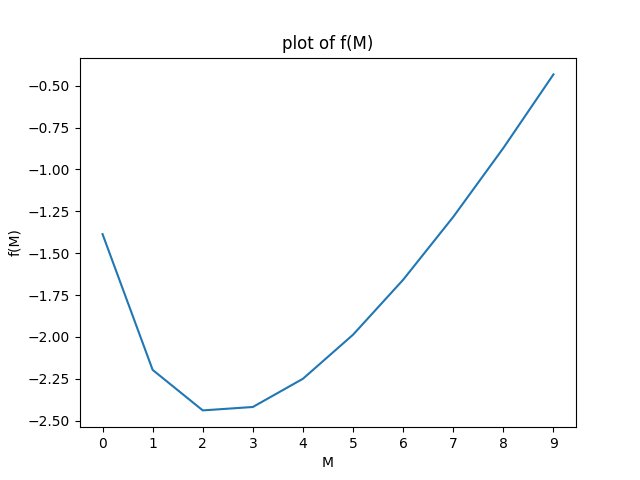
\includegraphics[scale=1]{fM.png} }
	\caption{plot of f(M)}\label{fMplot}
\end{figure}

\end{document}
